% Options for packages loaded elsewhere
\PassOptionsToPackage{unicode}{hyperref}
\PassOptionsToPackage{hyphens}{url}
\PassOptionsToPackage{dvipsnames,svgnames,x11names}{xcolor}
%
\documentclass[
  letterpaper,
  DIV=11,
  numbers=noendperiod]{scrartcl}

\usepackage{amsmath,amssymb}
\usepackage{lmodern}
\usepackage{iftex}
\ifPDFTeX
  \usepackage[T1]{fontenc}
  \usepackage[utf8]{inputenc}
  \usepackage{textcomp} % provide euro and other symbols
\else % if luatex or xetex
  \usepackage{unicode-math}
  \defaultfontfeatures{Scale=MatchLowercase}
  \defaultfontfeatures[\rmfamily]{Ligatures=TeX,Scale=1}
\fi
% Use upquote if available, for straight quotes in verbatim environments
\IfFileExists{upquote.sty}{\usepackage{upquote}}{}
\IfFileExists{microtype.sty}{% use microtype if available
  \usepackage[]{microtype}
  \UseMicrotypeSet[protrusion]{basicmath} % disable protrusion for tt fonts
}{}
\makeatletter
\@ifundefined{KOMAClassName}{% if non-KOMA class
  \IfFileExists{parskip.sty}{%
    \usepackage{parskip}
  }{% else
    \setlength{\parindent}{0pt}
    \setlength{\parskip}{6pt plus 2pt minus 1pt}}
}{% if KOMA class
  \KOMAoptions{parskip=half}}
\makeatother
\usepackage{xcolor}
\setlength{\emergencystretch}{3em} % prevent overfull lines
\setcounter{secnumdepth}{-\maxdimen} % remove section numbering
% Make \paragraph and \subparagraph free-standing
\ifx\paragraph\undefined\else
  \let\oldparagraph\paragraph
  \renewcommand{\paragraph}[1]{\oldparagraph{#1}\mbox{}}
\fi
\ifx\subparagraph\undefined\else
  \let\oldsubparagraph\subparagraph
  \renewcommand{\subparagraph}[1]{\oldsubparagraph{#1}\mbox{}}
\fi


\providecommand{\tightlist}{%
  \setlength{\itemsep}{0pt}\setlength{\parskip}{0pt}}\usepackage{longtable,booktabs,array}
\usepackage{calc} % for calculating minipage widths
% Correct order of tables after \paragraph or \subparagraph
\usepackage{etoolbox}
\makeatletter
\patchcmd\longtable{\par}{\if@noskipsec\mbox{}\fi\par}{}{}
\makeatother
% Allow footnotes in longtable head/foot
\IfFileExists{footnotehyper.sty}{\usepackage{footnotehyper}}{\usepackage{footnote}}
\makesavenoteenv{longtable}
\usepackage{graphicx}
\makeatletter
\def\maxwidth{\ifdim\Gin@nat@width>\linewidth\linewidth\else\Gin@nat@width\fi}
\def\maxheight{\ifdim\Gin@nat@height>\textheight\textheight\else\Gin@nat@height\fi}
\makeatother
% Scale images if necessary, so that they will not overflow the page
% margins by default, and it is still possible to overwrite the defaults
% using explicit options in \includegraphics[width, height, ...]{}
\setkeys{Gin}{width=\maxwidth,height=\maxheight,keepaspectratio}
% Set default figure placement to htbp
\makeatletter
\def\fps@figure{htbp}
\makeatother

\KOMAoption{captions}{tableheading}
\makeatletter
\makeatother
\makeatletter
\makeatother
\makeatletter
\@ifpackageloaded{caption}{}{\usepackage{caption}}
\AtBeginDocument{%
\ifdefined\contentsname
  \renewcommand*\contentsname{Table of contents}
\else
  \newcommand\contentsname{Table of contents}
\fi
\ifdefined\listfigurename
  \renewcommand*\listfigurename{List of Figures}
\else
  \newcommand\listfigurename{List of Figures}
\fi
\ifdefined\listtablename
  \renewcommand*\listtablename{List of Tables}
\else
  \newcommand\listtablename{List of Tables}
\fi
\ifdefined\figurename
  \renewcommand*\figurename{Figure}
\else
  \newcommand\figurename{Figure}
\fi
\ifdefined\tablename
  \renewcommand*\tablename{Table}
\else
  \newcommand\tablename{Table}
\fi
}
\@ifpackageloaded{float}{}{\usepackage{float}}
\floatstyle{ruled}
\@ifundefined{c@chapter}{\newfloat{codelisting}{h}{lop}}{\newfloat{codelisting}{h}{lop}[chapter]}
\floatname{codelisting}{Listing}
\newcommand*\listoflistings{\listof{codelisting}{List of Listings}}
\makeatother
\makeatletter
\@ifpackageloaded{caption}{}{\usepackage{caption}}
\@ifpackageloaded{subcaption}{}{\usepackage{subcaption}}
\makeatother
\makeatletter
\@ifpackageloaded{tcolorbox}{}{\usepackage[many]{tcolorbox}}
\makeatother
\makeatletter
\@ifundefined{shadecolor}{\definecolor{shadecolor}{rgb}{.97, .97, .97}}
\makeatother
\makeatletter
\makeatother
\ifLuaTeX
  \usepackage{selnolig}  % disable illegal ligatures
\fi
\IfFileExists{bookmark.sty}{\usepackage{bookmark}}{\usepackage{hyperref}}
\IfFileExists{xurl.sty}{\usepackage{xurl}}{} % add URL line breaks if available
\urlstyle{same} % disable monospaced font for URLs
\hypersetup{
  pdftitle={New York's Streetside Casualties},
  pdfauthor={Drew LoPolito and Mitch Harrison},
  colorlinks=true,
  linkcolor={blue},
  filecolor={Maroon},
  citecolor={Blue},
  urlcolor={Blue},
  pdfcreator={LaTeX via pandoc}}

\title{New York's Streetside Casualties}
\usepackage{etoolbox}
\makeatletter
\providecommand{\subtitle}[1]{% add subtitle to \maketitle
  \apptocmd{\@title}{\par {\large #1 \par}}{}{}
}
\makeatother
\subtitle{An explanatory analysis of NYC car accidents}
\author{Drew LoPolito and Mitch Harrison}
\date{}

\begin{document}
\maketitle
\ifdefined\Shaded\renewenvironment{Shaded}{\begin{tcolorbox}[borderline west={3pt}{0pt}{shadecolor}, sharp corners, interior hidden, enhanced, frame hidden, breakable, boxrule=0pt]}{\end{tcolorbox}}\fi

\hypertarget{introduction}{%
\section{Introduction}\label{introduction}}

\hypertarget{dataset}{%
\subsection{Dataset}\label{dataset}}

Our dataset is composed of harvested and compiled data from New York
City Police Department (NYPD) open access data on all police reported
motor vehicle collisions (MVC) in all five boroughs of New York City
from July 1st, 2012 through April 24th, 2023. The police report from
which individual MVC observations in our dataset hail (MV104-AN) is
required to be filled out for MVC where someone is injured or killed, or
which result in at least \$1,000 of total property damage. Notably, only
one MV104-AN form is filled out for all involved in an accident, meaning
each observation in our dataset represents a unique MVC.

Our initial dataset contained approximately 1.9 million observations,
found
\href{https://www.kaggle.com/datasets/utkarshx27/motor-vehicle-collisions?resource=download}{here}.
This was too large to push to git, so we sampled 10,000 observations
from the dataset completely at random (code shown in Methods). The
original dataset, as well as our randomly sampled dataset, contained
data on crashes involving 1 to 5 motorists, however, 93\% of crashes in
the dataset occurred between 2 or fewer motorists (98\% between 3 or
fewer and 100\% between 4 or fewer). Due to high levels of missingness
in crashes with 3 or more motorists, as well as their low real-world
frequency in New York City (where the kind of highway pile-ups which
generate MVC with 3 or more motorists aren't generally observed), we
decided to examine exclusively MVC between 2 or fewer motorists, which
brought our total number of observations down to approximately 9,300.

We created a number of new variables by manipulating the dataset, as
well as re-categorizing/cleaning some of the existing variables for
practical use in modeling (for example, the original variables for
factors contributing to the accident for each motorist and vehicle type
of each motorist contained roughly 100 categories).

The following are the variables of interest from our dataset, with new
or re-categorized variables noted:

\texttt{crash\_date}: the date on which the MVC occurred.

\texttt{crash\_day}: a categorical variable corresponding to the day of
the week on which the MVC occurred, generated from the original
\texttt{crash\_date} variable.

\texttt{yday}: a numeric variable ranging from 1 to 365 corresponding to
the numerical day of the year on which the MVC occurred.

\texttt{crash\_time} the time (in 24-hr time) at which the MVC occurred.

\texttt{time\_day}: a categorical variable with levels of ``morning,''
``afternoon,'' ``evening,'' and ``night'' corresponding to the time of
day at which a MVC occurred. This variable was generated from the
\texttt{crash\_time} variable, with ``morning'' from 5 AM to 12 PM,
``afternoon'' from 12 PM to 5 PM, ``evening'' from 5 PM to 9 PM, and
``night'' from 9 PM to 5 AM.

\texttt{num\_casualties}: a numeric variable corresponding to the number
of casualties, i.e., injuries or fatalities, resulting from an MVC. This
was generated from the original \texttt{number\_of\_persons\_injured}
and \texttt{number\_of\_persons\_killed} variables.

\texttt{has\_casualty}: a binary variable corresponding to whether or
not a MVC resulted in at least one casualty.

\texttt{vtype1} and \texttt{vtype2}: categorical variables corresponding
to the types of each vehicle (if applicable) involved in the crash, with
categories of ``Commercial vehicles,'' ``Passenger vehicles,''
``Motorcycles,'' ``Non-Motor Vehicle,'' and ``Other/Unknown.''

\texttt{factor1} and \texttt{factor2}: categorical variables
corresponding any notable factors which were listed as potentially
contributing to the crash (if applicable), with categories of
``Aggressive/Reckless Driving,'' ``Distraction/Inattention/Fatigue,''
``Failure to Obey Traffic Signs/Signals/Rules,'' ``Impaired,'' ``Other
Technical/Mechanical Factors,'' and ``Other/Unknown.''

Our primary research question of interest is whether an accident having
casualties or not depends on the type(s) of

\hypertarget{read-datalibraries}{%
\section{Read Data/Libraries}\label{read-datalibraries}}

\hypertarget{methodology}{%
\section{Methodology}\label{methodology}}

To explore the factors that lead to casualties in car accidents, we will
construct a binary logistic regression model. For the purposes of this
analysis, we define ``casualties'' as injuries or fatalities, not just
fatalities. We are only examining accidents involving two or fewer
vehicles, which account for over 90\% of accidents while avoiding the
complexities involved with correcting for several vehicle types at once.

We anticipate that the vehicle type involved in the accident will play a
significant role, but our dataset has over 100 individual vehicle types.
To simplify our model and avoid overfitting, we consolidated these into
five larger categories: passenger vehicles, commercial vehicles,
motorcycles, non-motor vehicles, and others/unknown. We also anticipated
a significant impact on accident severity by reason for the accident.
Specifically, we wanted to investigate impaired driving to other causes.
Like the vehicle type, however, we risked overfitting and
over-complicating our model because of the sheer number of accident
causes. Like our vehicle type variable, we consolidated accident causes
into five categories: impaired, distraction/inattention/fatigue,
aggressive/reckless driving, failure to obey traffic
signs/signals/rules, technical/mechanical failures, and other/unknown.

After consolidating categories, we investigate both the time of day and
the day of the year at which an accident occurred. Grouping by day of
the week, we find that the time at which injuries with casualties occur
varies, with fewer casualties around 5:00 pm and later at night during
the weekend. Because of this difference, we include both the time of day
and weekday in our model.

The day of the year (as measured by the number of days after January
1st, i.e., ``Julian Day'') is also included. During exploratory
analysis, we found that accidents had disproportionately few casualties
in the winter months and more around the middle of the year. Because of
this difference, we include the day of the year as a predictor in our
model.

We hoped to include the borough as a predictor but could not. So many
observations were missing a value for the borough that including it in
our complete-case model would have dropped a substantial portion of our
overall dataset. If we could confirm that the borough data was MCAR,
then we wouldn't be concerned about the final accuracy of our model.
However, because we could not verify the missingness mechanism (and due
to the general rarity of MCAR data that isn't explicitly designed as
such), we do not include the borough in which the accident occurs in our
model.

While we hoped that the zip code might provide valuable explanatory
insight, we found two issues with its inclusion in our model: first,
there are 100 unique zip codes in the dataset. As a categorical
variable, this would make our model much more complex to calculate and
communicate. Second, the proportion of accidents with casualties is
approximately normally distributed around a median of 1.191. Therefore,
specific zip codes are both unlikely to make an appreciable difference
in an explanatory model and are highly likely to increase its complexity
dramatically. Thus, we do not include zip code in our final model.

We also thought that some streets could have a disproportionately high
casualty rate and thereby have a statistically significant impact on our
model. However, we ran into many of the same problems that we did with
zip codes. In the 10,000 observations we selected from the larger
dataset, there were over 1000 unique streets, many of which had minimal
accidents. To combat these small number of observations, we used LaPlace
succession, adding one to each of the number of accidents and making it
a non-casualty accident. This technique allowed us to correct for low
accident counts. After applying LaPlace succession, we found that the
large majority of streets had no casualties at all, and the remainder
were distributed around 0.25. Because of the massive complexity that
adding a 1000-level categorical variable would add to our model,
combined with an unremarkable distribution of accident proportion after
applying LaPlace succession, we are not including streets as a predictor
in our final model.

\hypertarget{data-wrangling}{%
\section{Data Wrangling}\label{data-wrangling}}

\begin{verbatim}
[1] "NULL"
\end{verbatim}

\begin{verbatim}
NULL
\end{verbatim}

\begin{verbatim}
NULL
\end{verbatim}

\begin{verbatim}
# A tibble: 1 x 1
      n
  <int>
1  2823
\end{verbatim}

\begin{verbatim}
# A tibble: 1 x 1
      n
  <int>
1  1920
\end{verbatim}

\begin{verbatim}
# A tibble: 1 x 1
      n
  <int>
1     8
\end{verbatim}

\begin{verbatim}
# A tibble: 1 x 1
      n
  <int>
1   374
\end{verbatim}

\begin{verbatim}
# A tibble: 1 x 1
      n
  <int>
1   112
\end{verbatim}

\begin{verbatim}
# A tibble: 1 x 1
      n
  <int>
1    37
\end{verbatim}

\begin{verbatim}
# A tibble: 1 x 1
      n
  <int>
1    15
\end{verbatim}

\begin{verbatim}
# A tibble: 1 x 1
      n
  <int>
1     8
\end{verbatim}

\begin{verbatim}
# A tibble: 1 x 1
      n
  <int>
1     4
\end{verbatim}

\hypertarget{exploratory-analysis}{%
\section{Exploratory Analysis}\label{exploratory-analysis}}

\hypertarget{time-of-day}{%
\subsection{Time of Day}\label{time-of-day}}

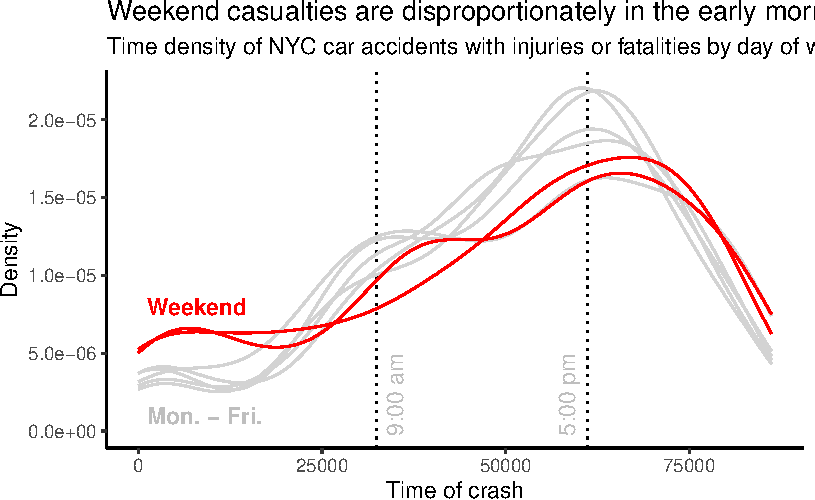
\includegraphics{project_files/figure-pdf/viz-time-density-1.pdf}

Of accidents with one or more casualties, those happening on Saturdays
and Sundays appear to occur disproportionately late at night and with a
notably smaller peak around 5:00 pm. While there is variance around the
weekend, the general pattern stays the same between all seven days. To
account for this, we will introduce a random effect based on the days of
the week to allow information sharing between them. We anticipate that
our model's performance will benefit from such a change, and this random
effect will end up in the final model after performance evaluation.

\hypertarget{day-of-the-year}{%
\subsection{Day of the year}\label{day-of-the-year}}

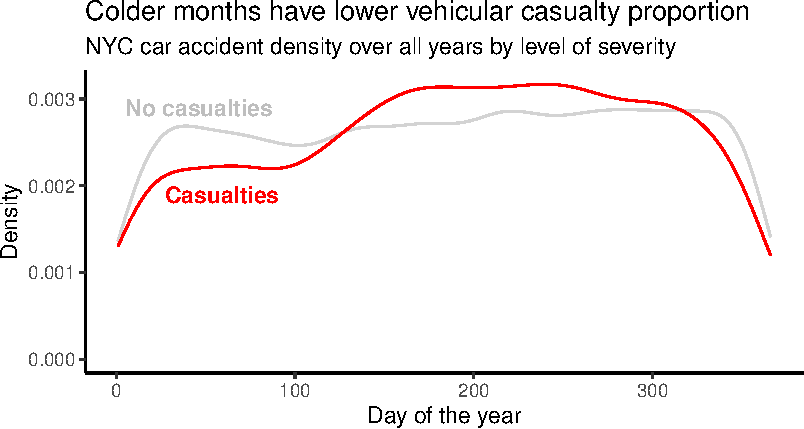
\includegraphics{project_files/figure-pdf/viz-density-severity-day-of-year-1.pdf}

The variance in density between levels of severity of accidents through
all years is relatively low. However, we see disproportionately severe
accidents around the late summer/early spring months and minor accidents
in the early winter months. This difference is enough to include it as a
potential predictor of interest in our final model.

\hypertarget{borough}{%
\subsection{Borough}\label{borough}}

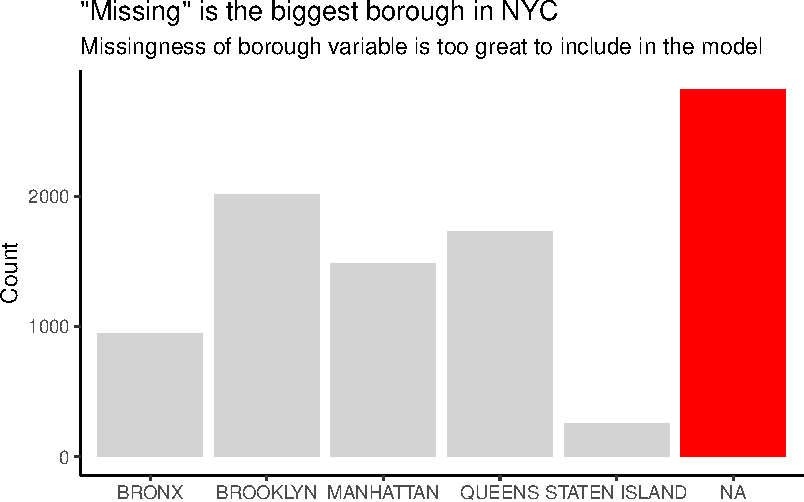
\includegraphics{project_files/figure-pdf/viz-hist-by-street-1.pdf}

We have far too many missing values to include borough in our model. If
we could verify that borough was Missing Completely At Random (MCAR), we
could include it in our complete-case model. Still, unfortunately, we
are unable to verify the missingness mechanism and are therefore
uncomfortable with possible performance impacts by using borough in our
final model.

\hypertarget{zip-codes}{%
\subsection{Zip codes}\label{zip-codes}}

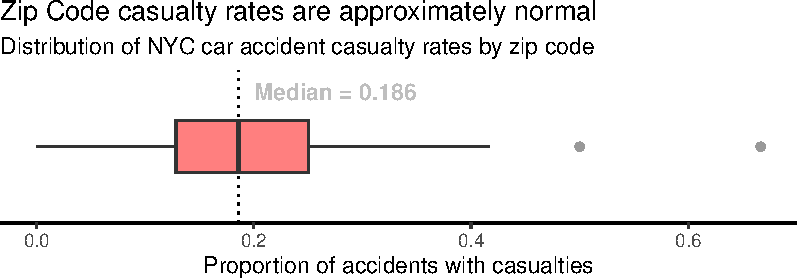
\includegraphics{project_files/figure-pdf/viz-zip-code-box-1.pdf}

Building a box plot to observe the distribution of accident proportion
by zip code, we see that casualty rates are approximately normally
distributed about a median of 0.191. Because of the large absolute
number of zip codes in the dataset and the unlikely impact of a normally
distributed proportion having a significant impact on the model, we will
not use zip code as a predictor in the final model.

\hypertarget{streets}{%
\subsection{Streets}\label{streets}}

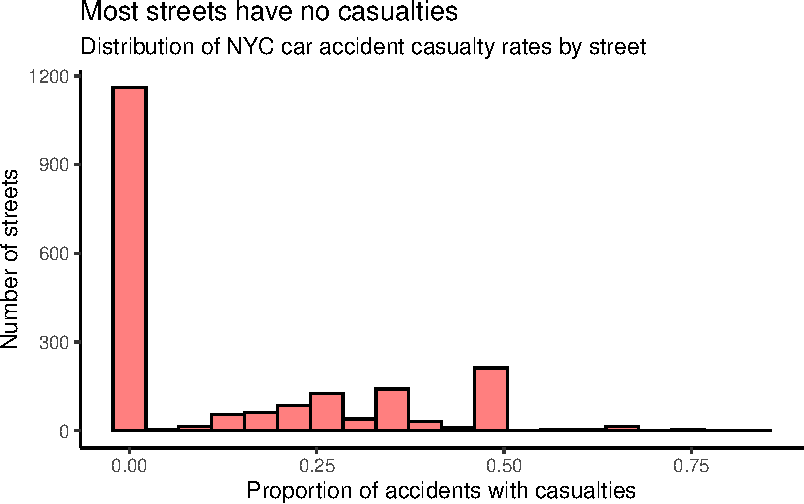
\includegraphics{project_files/figure-pdf/viz-streets-hist-1.pdf}

After applying LaPlace succession, we see that the vast majority of
accidents had no casualties, and most others were distributed around
0.25, with another peak around 0.5, partially due to the mathematical
consequences of LaPlace succession. Because so many streets followed an
unremarkable distribution and because adding street as a predictor would
introduce massive model complexity, we will not use the street on which
an accident occurs as a predictor in the final model.

\newpage{}

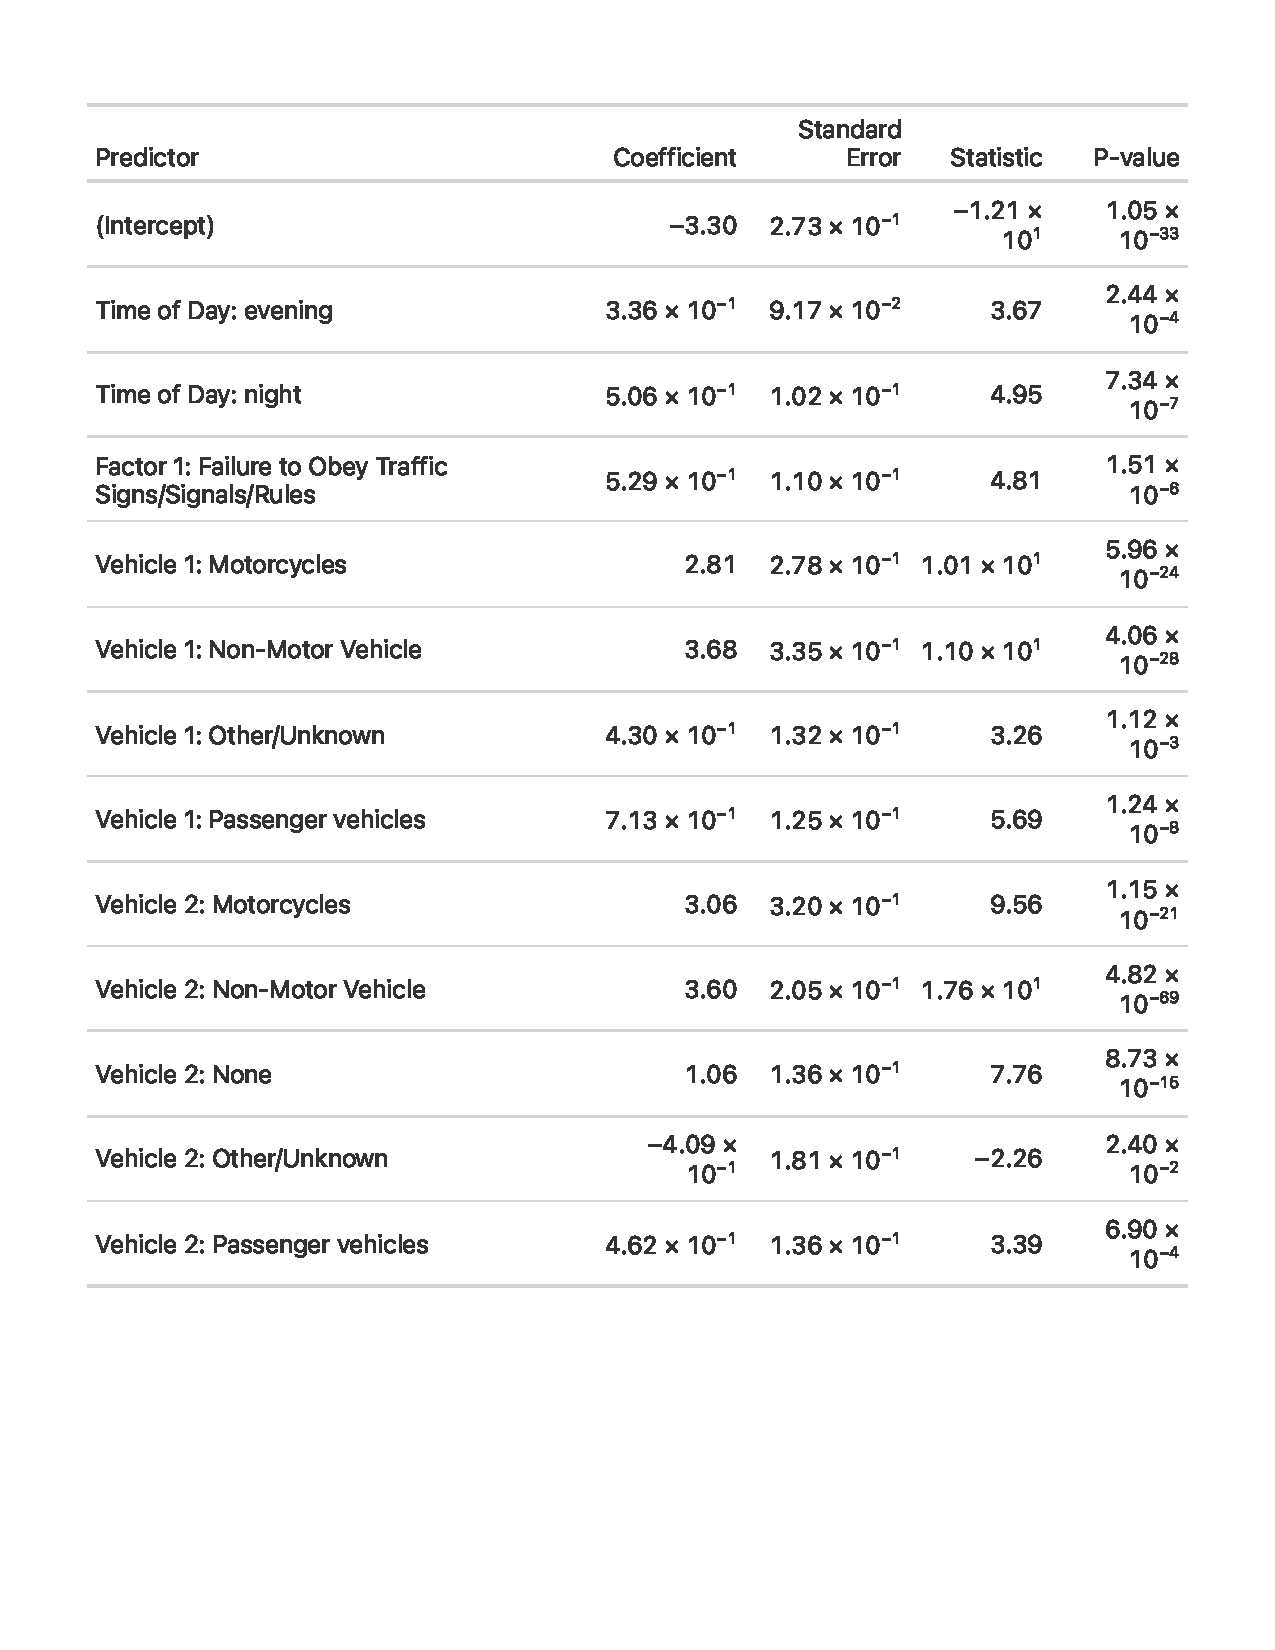
\includegraphics{table1.pdf} 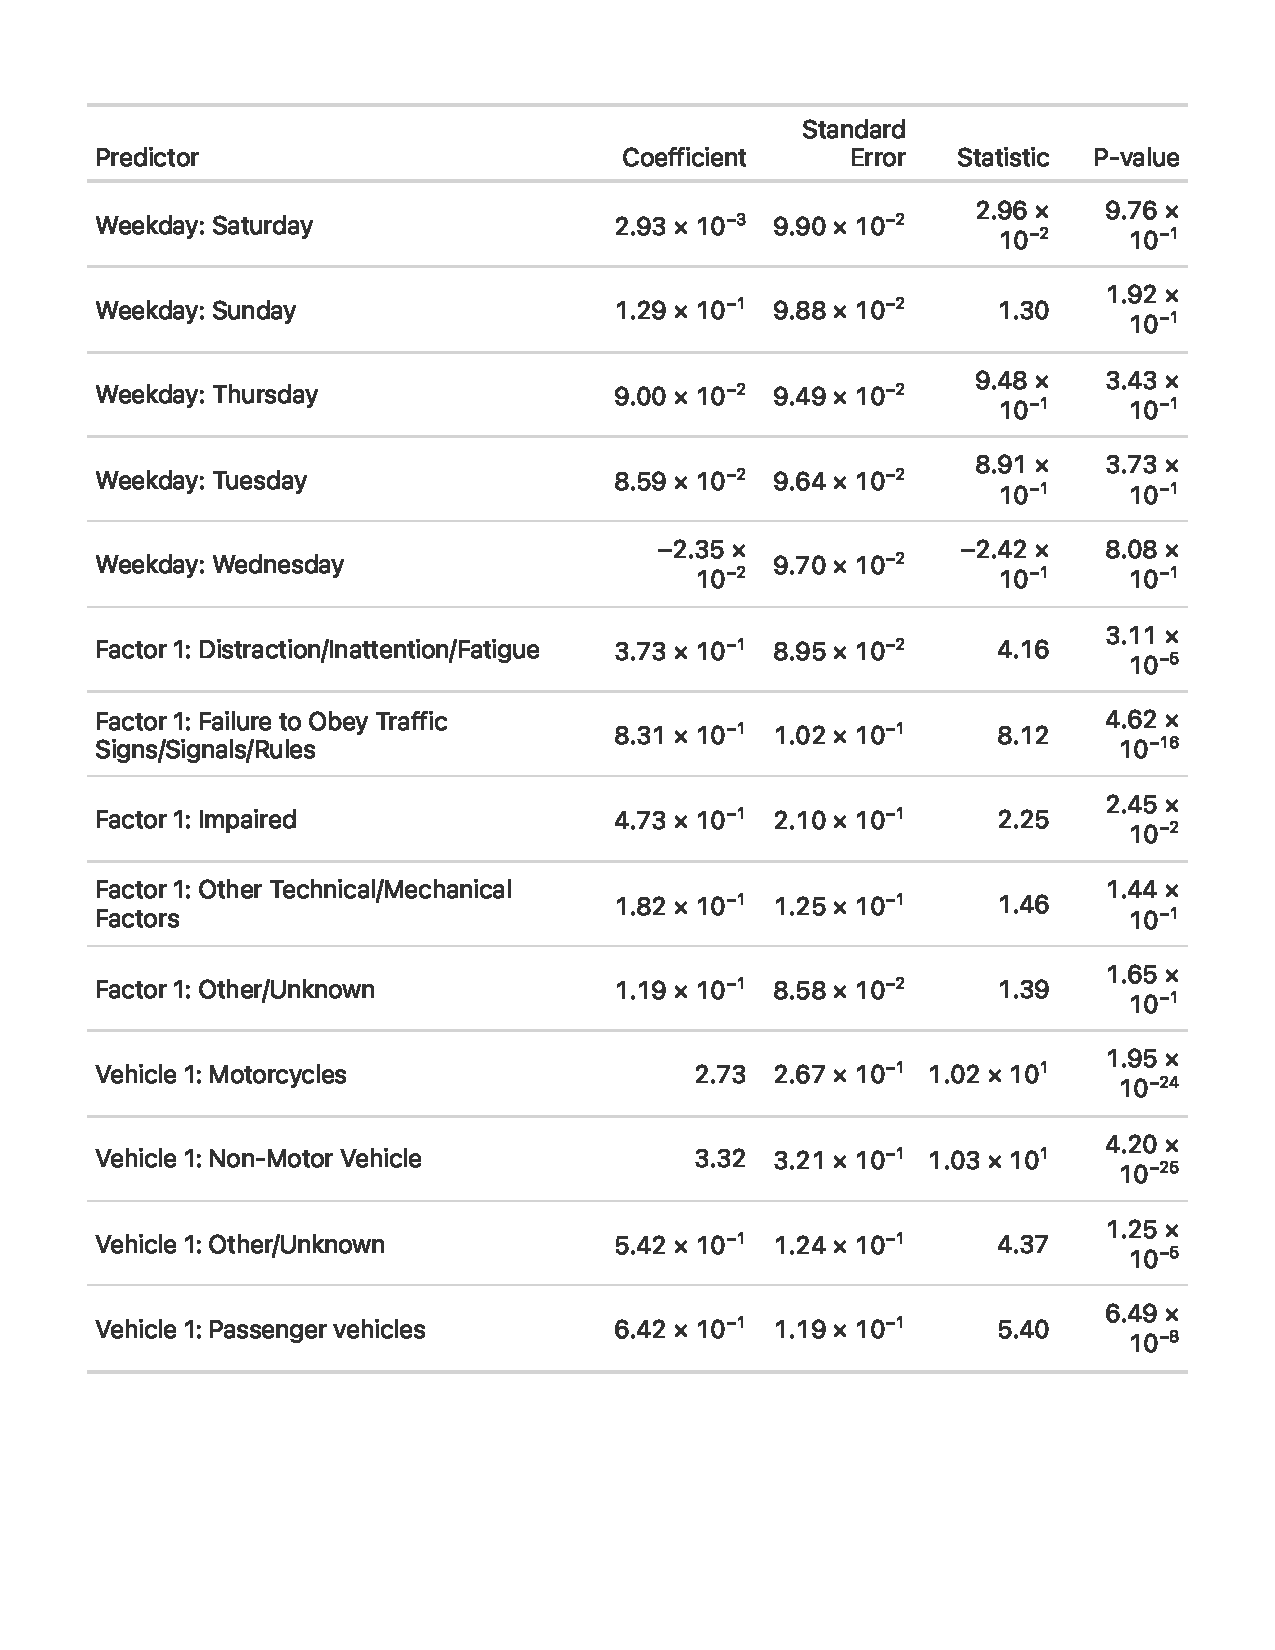
\includegraphics{table2.pdf}

\newpage{}

\hypertarget{results}{%
\section{Results}\label{results}}

\hypertarget{discussion}{%
\section{Discussion}\label{discussion}}



\end{document}
